\documentclass[12pt,letterpaper,noanswers]{exam}
\usepackage[usenames,dvipsnames,svgnames,table]{xcolor}
\usepackage[margin=0.9in]{geometry}
\renewcommand{\familydefault}{\sfdefault}
\usepackage{multicol}
\pagestyle{head}
\header{AM 108 Class 21}{}{Lorenz system}
\runningheadrule
\headrule
\usepackage{graphicx} % more modern
\usepackage{amsmath} 
\usepackage{amssymb} 
\usepackage{hyperref}
\usepackage{tcolorbox}

\begin{document}
 \pdfpageheight 11in 
  \pdfpagewidth 8.5in

\noindent 




\begin{itemize}
\item Problem set 08 is due Friday October 30th.
\end{itemize}

\hrule
\vspace{0.2cm}



\noindent\textbf{Project Teams}

Names removed


\noindent \textbf{Teams 3 and 4}: Post screenshots of your work to the course Google Drive today.  Include words, labels, and other short notes that might make those solutions useful to you or your classmates.  Find the link in Canvas (or here: \url{https://drive.google.com/drive/u/0/folders/1GcpwvKHD4tMecpFQ4lNxN_r5Ylj7YHbd})


\vspace{0.2cm}

\hrule
\vspace{0.2cm}

\noindent\textbf{Big picture}

Simple nonlinear dynamical systems in 3 variables can have surprisingly complicated and hard to predict long term behavior.  The Lorenz '63 system is an important example of such a system: it is the system in which this kind of hard-to-predict behavior was first characterized.


\vspace{0.2cm}
\hrule
\vspace{0.2cm}

\noindent \textbf{Extra vocabulary / extra facts:}
\begin{tcolorbox}

A dynamical system is \textbf{dissipative} if volumes (or areas) in phase space are decreased under the forward action of the flow (for all forward times).  For physical systems, dissipation is associated with energy loss.

A dynamical system is \textbf{volume contracting} when the surface, $\partial V$, of a region $V$ moves under the action of the flow in such a way that the enclosed volume decreases with time. %A patch of surface sweeps out the volume $dA(\underline{f}\cdot\underline{n}dt$ in time $dt$.  We have $V(t+dt) = V(t)+\int_S\underline{f} dt\cdot\underline{n}\ dA$ so $\dot V = \frac{V(t+dt)-V(t)}{dt} = \int_S \underline{f}\cdot\underline{n}dA = \int_V \nabla\cdot \underline{f} dV$ by the divergence theorem.

When the \textbf{divergence} of the vector field is negative everywhere, volumes will be contracted by the flow.  \emph{See section 9.2 for details}.

In a dynamical system in 3d, \textbf{closed trajectories can be saddle-like}: they can have two spiraling directions that are stable and one non-spiraling direction that is unstable.  Or they might have two spiraling directions that are unstable and one that is stable.

When a dynamical system is volume contracting, it will not have repelling fixed points or repelling limit cycles.  Those would create small regions of volume expansion.  Limit cycles and fixed points will be stable or saddle-type.

A dynamical system in $n$-dimensions has $n$ different \textbf{Lyapunov exponents}. Imagine creating a tiny (infinitesimal) sphere of perturbed initial conditions at a point in the phase space.  The Lyapunov exponents describe the evolution of the sphere into an ellipsoid under the local action of the flow.  In the Lorenz system the sphere is squished in some directions (negative Lyapunov exponents) and stretched in one direction (positive Lyapunov exponent).

Often the term \textbf{Lyapunov exponent} is used to refer to the largest one.

\end{tcolorbox}

\begin{tcolorbox}
\textbf{Some properties of the Lorenz '63 system}

\begin{align*}
\dot x &= -\sigma x + \sigma y \\
\dot y &= rx - y - xz \\
\dot z &= xy - bz
\end{align*}

This system has just two \textbf{quadratic nonlinearities} in the equations ($-xz$ and $xy$).

There is a spherical \textbf{trapping region}, $x^2+y^2 + (z-r-\sigma)^2 = C$ (for $C$ sufficiently large) and all trajectories eventually enter it. 

This system is (strongly) \textbf{volume contracting}.

Two trajectories that start very close to each other will \textbf{diverge}, separating exponentially fast.
\end{tcolorbox}

\vspace{0.2cm}
\hrule
\vspace{0.2cm}

\textbf{Addressing your questions}
\begin{enumerate}
    \item Returning to timing of the limit cycle in the homoclinic bifurcation: $\mathcal{O}(\ln \mu)$ vs $T\propto \ln \frac{1}{\mu}$
    \item What was Steve's argument about quasiperiodicity and a torus?
    \item Steve mentioned that we never truly know where we are starting.  Wasn't this true in 2D as well?
    \item When we linearize, we just dropped the quadratic terms.  Is this equivalent to finding the Jacobian?  When can we do this?
        \item Steve looked only at $\dot x$ and $\dot y$.  Will we sometimes need a Jacobian for all three variables?
        \item With the Hopf bifurcation, how was its parameter value determined and how do we know it was subcritical?
        \item What happens to the system at large $r$?
    \item What does this strange attractor mean?
    \item How does the Lorenz system relate to other chaotic systems?
    \item What if the symmetry were removed from this system?  Could there still be chaotic behavior?
    \item Which parameters in the Rayleigh-Benard system affect what conditions?

    
\end{enumerate}

\vspace{0.2cm}
\hrule
\vspace{0.2cm}


\noindent\textbf{Skill Check C22 practice}
\begin{questions}
\item Retake of skill check C19: finding the parameter value associated with a Hopf bifurcation


\item In the plot on the left, the $x$-coordinate is shown vs time for two trajectories of the Lorenz system.  The two trajectories started with a separation of $\delta_{old}(0) = 10^{-4}$ in their initial conditions.

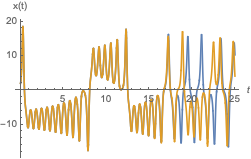
\includegraphics[width=0.45\textwidth]{img/C24-2019-11-01p1.png}\hfill
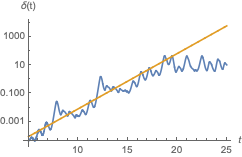
\includegraphics[width=0.45\textwidth]{img/C24-2019-11-01p2.png}

The evolution of the separation of the two trajectories, $\delta(t)$, is shown in blue on the plot on the left.  This separation grows exponentially (until it reaches approximately the size of the attractor).  A reference curve, $f(t) = ce^{0.9t}$, is plotted in orange. 


Think of the orange trajectory as the ``truth'' and the blue trajectory as a prediction.  If we'd like the prediction to be as good at time $20$ as it currently is at time $10$, how much smaller would $\delta(0)$ need to become (i.e. what is $\delta_{new}(0)$)?  As an approximation, assume $\delta(t) =\delta(0) e^{0.9t}$.

\emph{Note: $e^3\approx 20$ if you'd like to find an approximate value.}

\end{questions}

\vspace{0.2cm}

\hrule
\vspace{0.2cm}

\noindent\textbf{Skill check C22 practice solution}

We have $\delta(10) = \delta_{old}(0) e^{0.9*10}$.  We want $\delta(20) = \delta_{old}(0)e^{0.9*10}$ where $\delta(20) = \delta_{new}(0)e^{0.9*20}$.

$\delta_{old}(0) e^{0.9*10} = \delta_{new}(0)e^{2*0.9*10}$.

$\Rightarrow \delta_{old}(0) = \delta_{new}(0)e^{0.9*10}$ so $\delta_{new}(0) = \delta_{old}(0)*e^{-9}\approx 10^{-4}/20/20/20 = 10^{-7}/8\approx 10^{-8}$.

Four orders of magnitude smaller to double the prediction time...

\vspace{0.2cm}

\hrule
\vspace{0.2cm}
\noindent\textbf{Questions}

\noindent \ \ 0.  Introduce yourself to your team (and write your names on the slide).

\begin{questions}

\question (8.6.1: ``Oscillator death'' and bifurcations on a torus)  We have worked with models of a single oscillator following a reference oscillator but haven't had the chance to work with a model where each oscillator responds to the other oscillator.

This model is from Ermentrout and Kopell (1990), where the authors were considering a system of interacting neural oscillators.  They developed a simple example with two interacting oscillators that captured many of the interaction properties they wanted for their neural system.  Specifically, they wanted to capture that coupling between oscillators can actually suppress oscillation (``oscillator death'') and lead to a steady state of the coupled system.  Here is their example model:
\begin{align*}
\dot{\theta_1} = &\ \omega_1 + \sin \theta_1 \cos\theta_2 \\
\dot{\theta_2} = &\ \omega_2 + \sin \theta_2 \cos\theta_1.
\end{align*}
The oscillators have a natural frequency, but they also are responding to each other.

There are a number of different behaviors possible in this system.
We will work to figure out the possible behaviors by identifying bifurcations and  plotting a stability diagram in $\omega_1\omega_2$ space.

\begin{parts}
\item Looking for fixed points of $\phi = \theta_1-\theta_2$ allows us to identify curves where $\theta_1 = \theta_2 + c$ where $c$ is a constant. 

Here, use both $\phi = \theta_1 - \theta_2$ (``phi'') and $\psi = \theta_1 + \theta_2$ (``psi'') to aid your analysis.  

If $\dot{\phi} = 0$ and $\dot{\psi} = 0$ (and only if this is true) then the system has a fixed point.  Why is that?
\item Find $\dot{\phi}$ and $\dot{\psi}$ equations.  \emph{Look up trig identities as needed.}
\item In what region of the $\omega_1\omega_2$ plane does the system have fixed points?
\item In what regions of the $\omega_1\omega_2$ plane does this system have $\dot{\phi} = 0$ or $\dot{\psi} = 0$ but not both?  Sketch a phase portrait in the $\theta_1\theta_2$ plane in such a case.
\end{parts} 

\item (8.4.1 - SNIPer bifurcation) Consider the system given by 
\begin{align*}
\dot{r} = &\ r(1-r^2) \\
\dot{\theta} = &\ \alpha - \sin\theta
\end{align*}
with $\alpha$ slightly greater than $1$, so we are on the verge of an infinite period bifurcation.
\begin{parts}
\item Sketch the phase portrait in the $xy$-plane.
\item In lecture we saw the approximate waveform for $x(t)$.  Recall that $x = r\cos\theta$, and plot $x$ vs $t$.
\item Also sketch the waveform for $y(t)$.
\item As $\alpha$ changes so that we pass through the bifurcation, how will the amplitude of the oscillation vary with $\alpha$?
\item Let $T$ be the period of the oscillation.  If we are at a point $(x_c, y_c)$ on the limit cycle, then after time $T$, we will return to the same point.  This return takes time $T = \int_0^T dt$.  We can rewrite this in terms of our angular position on the limit cycle, so \[T = \int_0^{2\pi} \frac{dt}{d\theta}d\theta = \int_0^{2\pi} \frac{1}{\alpha-\sin\theta}d\theta.\]

We want to determine how this period, $T$, scales with $\alpha$ as we approach the bifurcation.  The bifurcation occurs when $\alpha = 1$, so we actually want to know how the period scales with $\mu = \alpha - 1$.

It is possible to use a substitution ($u = \tan \frac{\theta}{2}$) to evaluate this integral exactly.  We just want the scaling though, so we'll use an approximation.

The bifurcation occurs when $\alpha = 1$ and the system state is $r = 1, \theta = \pi/2$ at the bifurcation point.  We assume that oscillator spends most of its time close to the bifurcation.  Let $\mu = \alpha -1$ and $x = \theta - \pi/2$.  Taylor expand $\dot{\theta}$ near the bifurcation.

\emph{You should find $\dot{x} = \mu + \frac{x^2}{2}$.}

\item Assuming that most time is spent near the bifurcation, $\displaystyle T \approx \int_{-\infty}^{\infty} \frac{1}{\mu + \frac{x^2}{2}}\ dx.$  We want to rewrite this integral as $T\approx f(\mu) \int_{-\infty}^{\infty} g(x) \ dx$.  If we're able to rewrite it in that form, then $\int_{-\infty}^{\infty} g(x) \ dx$ is a constant that does not depend on $\mu$ and $f(\mu)$ tells us the scaling (how the period varies with $\mu$).

Try pulling $\frac{1}{\mu}$ out of the integral.  That doesn't quite get rid of all of the $\mu$'s.  Next try a substitution.  Let $u = x/??$ so as to eliminate the $\mu$ in the denominator.  Complete the substitution to find $f(\mu)$.  How does the period of the oscillation depend on $\mu$?

\end{parts}

\item (Volume contraction) The Lorenz system is dissipative, meaning that volumes in the phase space are contracted under the flow.  Consider an arbitrary closed surface $S$.  This surface encloses a region $W$ that has volume $V$.  We can think of every point in $W$ as the initial condition of a trajectory.  Let each of them evolve forward in time (under the action of the dynamical system), let $W(t)$ be the set they evolve to at time $t$ (with surface $S(t)$.  The volume of the set is evolving in time!

%for time $\Delta t$, then the volume may change.  

How does the volume change with time?  

The divergence of a vector field is a measure of local contraction (negative sign) or local expansion (positive sign) under the action of the vector field.

The divergence theorem tells us that if we integrate the divergence over a region $W$, we learn about the net push of the vector field at the surface of the region.  

The action of the vector field is changing the size of our region.  For the size to change, the surface must be enclosing a growing or a shrinking volume.

Learning about the net push of the vector field at the surface tells us about the change in the volume.

Specifically:

$\displaystyle \dot{V} = \int_W \text{div }\vec{f}\ dV$ where $\vec f$ is the vector field given by the dynamical system.  
\begin{parts}
\item Find $\text{div }\vec f$ and argue that $\dot{V}$ is negative for the Lorenz system.  Use this to conclude that volumes contract.  When volumes in phase space are contracted under the action of the flow, we call a system \emph{dissipative}, so you are showing that the Lorenz system is a dissipative system.

\emph{Recall that $\text{div }\vec f = \nabla \cdot \vec f = \frac{\partial \dot x}{\partial x} + \frac{\partial \dot y}{\partial y} + \frac{\partial \dot z}{\partial z}$.}

\item Use $\dot V = \int_W \nabla \cdot \underline{f}\ dV$ to find $V(t)$ for this system.

\end{parts}

\end{questions}

\eject

1: prey: $x$, predator: $y$.  fixed points: $(0,0)$, $(1,0)$, and $(a,a-a^2)$.  classification: $(0,0)$ a saddle for $a>0$, $(1,0)$ a saddle for $0<a<1$, stable for $a>1$.  $(a,a-a^2)$ unstable for $0<a<\frac{1}{2}$, stable for $\frac{1}{2}<a<1$ and a saddle for $a>1$.  Hopf at $a_c = 1/2$.   At $a_c = 1$ two fixed points exchange stability (and collide) so transcritical.  frequency of oscillation is given by the imaginary part of the eigenvalues near $a_c$ so $\omega \approx \frac{1}{2\sqrt{2}}$. Stable limit cycle at $a = 0.46, 0.48$ and stable spiral at $0.52,0.54$ so appears to be supercritical.


2a: Assume $\dot \phi = 0$ and $\dot \psi = 0$.  Then $\dot \phi + \dot \psi = 2\dot \theta_1 = 0$ so $\theta_1$ is fixed and $\dot \psi - \dot\phi = 2\theta_2 = 0$ so $\theta_2$ is fixed.  Going the other direction, if $\dot\theta_1 = 0$ and $\dot\theta_2=0$ then their sum and their difference is zero as well.

2b: $\dot\phi = \omega_1 - \omega_2 + \sin\theta_1\cos\theta_2 - \sin\theta_2\cos\theta_1 = \omega_1-\omega_2 + \sin(\theta_1 - \theta_2) = \omega_1-\omega_2 + \sin(\phi).$

$\dot\psi = \omega_1 + \omega_2 + \sin\theta_1\cos\theta_2 + \sin\theta_2\cos\theta_1 = \omega_1+\omega_2 + \sin(\theta_1 + \theta_2) = \omega_1+\omega_2 + \sin(\psi).$

2c: fixed points when $\dot \phi = 0$ and $\dot\psi = 0$ so need $\vert\omega_1 - \omega 2\vert\leq 1$ and $\vert \omega_1+\omega_2 \leq 1$.  Draw the lines $\omega_1 -\omega_2 = 1$, $\omega_1-\omega_2 = -1$, $\omega_1+\omega_2 = 1$ and $\omega_1+\omega_2 =-1$.  These lines enclose a square region (tilted 45 degrees) centered around the origin where there are fixed points.

2d: $\dot\phi = 0$ but $\dot\psi$ happens for $-1\leq \omega_1 - \omega_2 \leq 1$ and $\omega_1+\omega_2 >1$ or $\omega_1+\omega_2 < -1$.  The region between the orange and green lines below is a region where one is zero but not both.  In the $\omega_1\omega_2$ plane there are four such regions.

Assume $\dot\phi = 0$. The systems are completely decoupled, so we can just think about the $\phi$ system.  There exists a steady state $\phi$ value, $\phi_s = c$ (and usually two: one stable and one unstable).  These correspond to a steady state relationship $\theta_1 = \theta_2 + c$.  So there are two closed orbits...

\begin{verbatim}
StreamPlot[{1 + Sin[x] Cos[y], 1.5 + Sin[y] Cos[x]}, {x, -Pi, 
  Pi}, {y, -Pi, Pi}, FrameLabel -> {"\[Theta]1", "\[Theta]2"}, 
 LabelStyle -> Medium]
\end{verbatim}

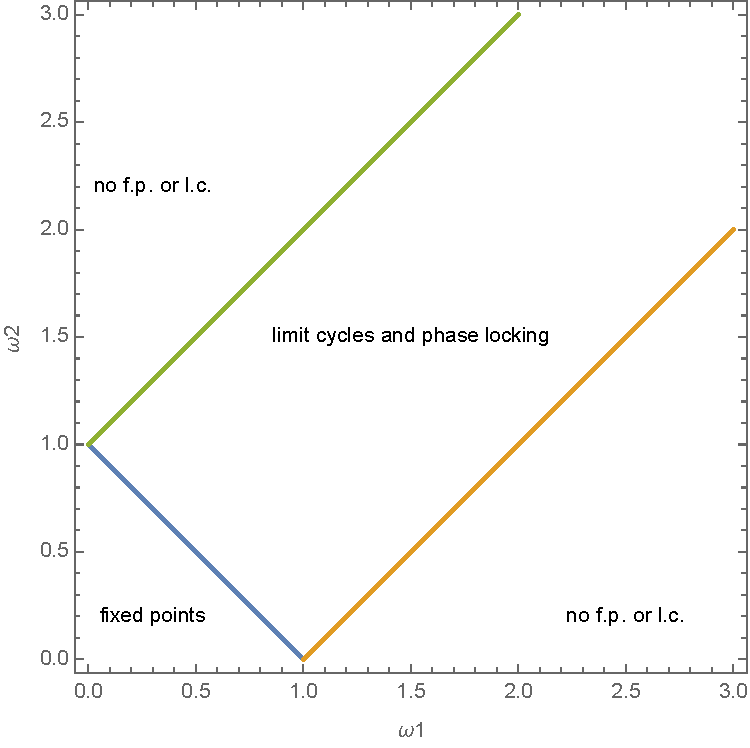
\includegraphics[scale=0.3]{img/C17plot.pdf}

2a: 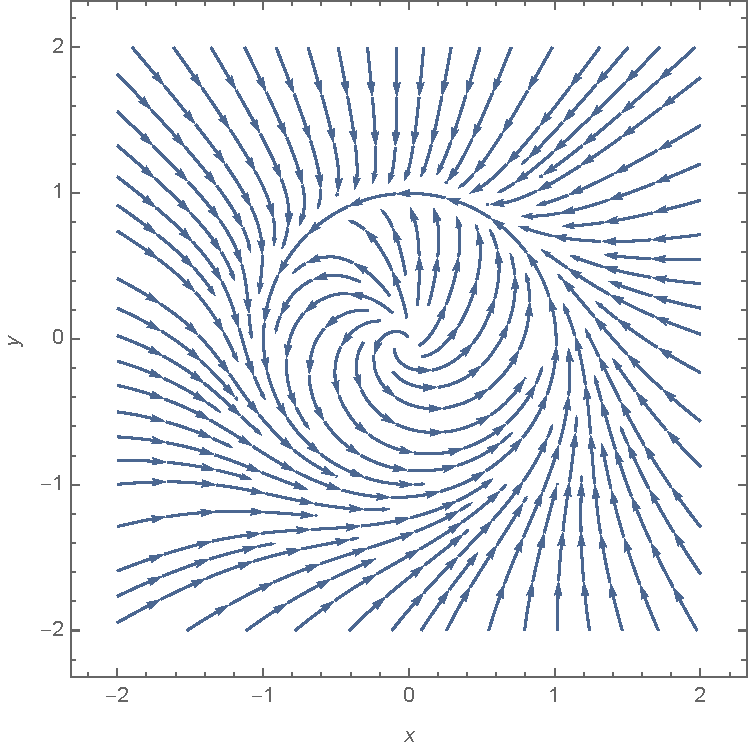
\includegraphics[width=2in]{img/C15p1.pdf}
2bc: 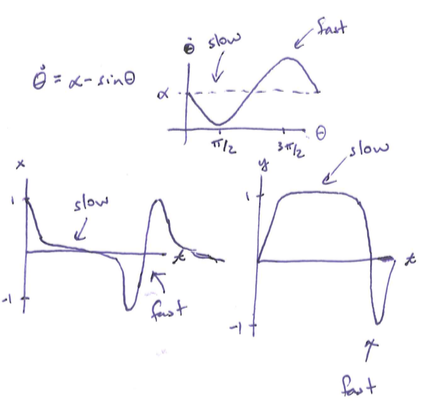
\includegraphics[width=4in]{img/S19C18p4.png}

Waveforms for $\mu = 1.1$ and $\mu = 1.01$. 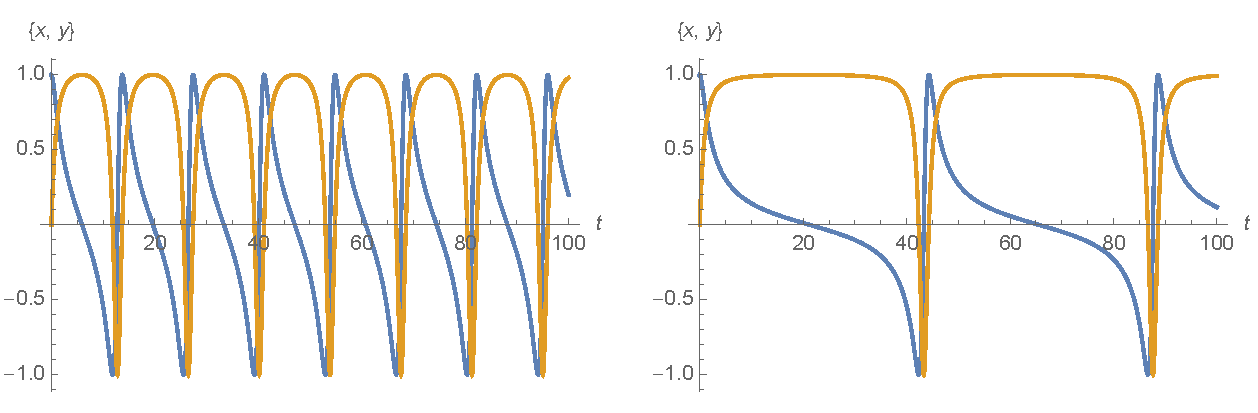
\includegraphics[width=4in]{img/InfinitePeriod.pdf}

2d: the amplitude is always about $1$, so not varying with $a$.
2e: Start with a linear approximation: $\dot \theta \approx \alpha - \sin\pi/2 + (\theta - \pi/2)f'(\pi/2) = \alpha -1 + (\theta -\pi/2)(-\cos \pi/2) = \alpha -1 = \mu$.  This isn't enough terms so go to quadratic order.  The next term is $\frac{1}{2}(\theta - \pi/2)^2f''(\pi/2) = \frac{1}{2} x^2 \sin \pi/2 = \frac{1}{2}x^2$.  $\dot \theta = \dot x \approx \mu + \frac{1}{2}x^2.$

2f: pull out $1/\mu$: $\displaystyle T \approx \frac{1}{\mu}\int_{\infty}^\infty \frac{1}{1+x^2/(2\mu)}dx$

change of variables: $u = x/\sqrt{2\mu}$ so $du = dx/\sqrt{2\mu}$.  $\displaystyle T \approx \frac{1}{\mu} \int_{\infty}^\infty \sqrt{2\mu}\frac{1}{1+u^2}du = \frac{1}{\sqrt{\mu}}\int_{\infty}^\infty \sqrt{2}\frac{1}{1+u^2}du$


3a: $\vec\nabla \cdot \vec f = -\sigma -1 -b < 0$.  This is a constant, so $\dot V = -(\sigma + 1 + b)\int_W dV = -(\sigma + 1 + b)V$.  3b: $\dot V = -(\sigma + 1 + b)V$ so $V(t) = V_0 e^{-(\sigma+1+b)t}.$
\end{document}